\iffalse
\documentclass[journal,10pt,twocolumn]{article}
\usepackage{graphicx}
\usepackage[margin=0.5in]{geometry}
\usepackage{amsmath}
\usepackage{array}
\usepackage{booktabs}
\usepackage{listings}
\providecommand{\norm}[1]{\left\lVert#1\right\rVert}
\providecommand{\abs}[1]{\left\vert#1\right\vert}
\usepackage{enumerate}
\let\vec\mathbf
\newcommand{\myvec}[1]{\ensuremath{\myvec{#1}}}
\newcommand{\mydet}[1]{\ensuremath{\begin{vmatrix}#1\end{vmatrix}}}
\providecommand{\brak}[1]{\ensuremath{\left(#1\right)}}
\lstset{
frame=single,
breaklines=true,
columns=fullflexible
}
\title{\textbf{Matrix Assignment}}
\author{A L U R U A J A Y}
\date{September 2022}
\begin{document}
\maketitle
\paragraph{\textit{Problem Statement} -
\fi
Find the equation of the tangent line to the curve
\begin{align}
y=x^2-2x+7
\end{align}
\begin{enumerate}
    \item parallel to the line $2x-y+9=0$.
    \item perpendicular to the line $5y-15x=13$.
\end{enumerate}
\solution
	\begin{figure}[!h]
		\centering
 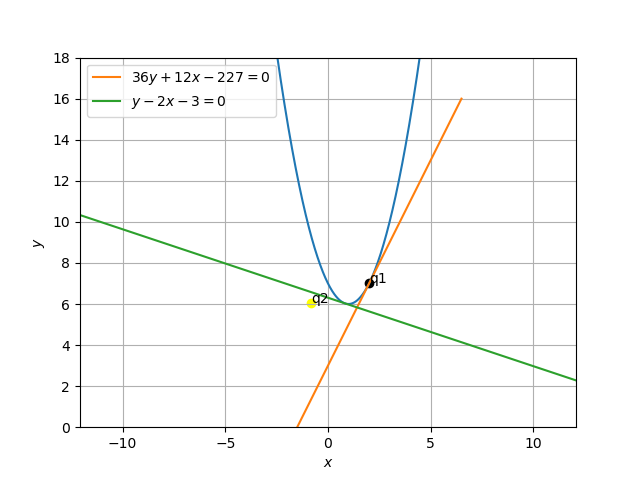
\includegraphics[width=\columnwidth]{chapters/12/6/3/15/figs/conic.png}
		\caption{}
		\label{fig:12/6/3/15}
  	\end{figure}
\iffalse

\section{Solution}
According to the question equation of a parabola is 
\vspace{0.3cm}\\
\begin{align}
y=x^2-2x+7
\end{align}
\vspace{0.3cm}\\
The standard equation of the parabola is given as :
\begin{align}
\vec{x}^{\top}\vec{V}\vec{x}+2\vec{u}^{\top}\vec{x}+f=0
\end{align}
\fi
The parameters of the given conic are
\begin{align}
\vec{V} =\myvec{
	1 & 0\\
	0 & 0
	},
    \vec{u}=-\myvec{
	1 \\
	\frac{1}{2}
	},
    f=7
    \end{align}
\begin{enumerate}
	\item In this case,  the normal vector
		\begin{align}\vec{n}_1 = \myvec{2 \\ -1}\end{align}
			Since 
$\vec{V}$ is not invertible,  
		%Then given the normal vector \begin{align}\vec{n}\end{align}\, 
	the point of contact is given by 
\eqref{eq:conic_tangent_q_eigen} resulting in 
		%the matrix equation
\iffalse
\vspace{0.3cm}\\
\begin{align}
    \myvec{(\vec{u}+k_1\vec{n}_1)^{\top} \\ \vec{V}}\vec{q}_1 = \myvec{-f \\ k_1\vec{n}_1- \vec{u}}
\end{align}
\fi
\begin{align}
\myvec{\myvec{-1 \\ -\frac{1}{2}} + \frac{1}{2}\myvec{2 \\ -1}^{\top} \vspace{0.3cm}\\ \myvec{
	1 & 0\\
	0 & 0\\
	}} \vec{q}_1 = \myvec{-7 \vspace{0.3cm}\\ \frac{1}{2}\myvec{2 \\ -1} - \myvec{-1 \\ -\frac{1}{2}}}
\end{align}
By solving the above equation, we can get the point of contact as
    \begin{align}
  \vec{q}_1=\myvec{
	2 \\
	7 \\
	}
\end{align}
The 
tangent equation is then obtained as
\begin{align}
      \vec{n}_1^{\top}(\vec{x}-\vec{q}_1) = 0
  \\
	\implies  \myvec{2 & -1}\vec{x}+3 = 0
\end{align}
\item 
	\iffalse
\subsection{perpendicular to the line 5y-15x=13}
\fi
In this case, 
		\begin{align}\vec{n}_2 = \myvec{1 \\ 3} \end{align}
	\iffalse
\begin{flushleft}
\begin{align}\vec{V}\end{align}\ is not invertible,Then given the normal vector \begin{align}\vec{n}\end{align}\, the point of contact to is given by the matrix equation
\vspace{0.3cm}\\
\begin{align}
    \myvec{(\vec{u}+k_2\vec{n}_2)^{\top} \\ \vec{V}}\vec{q}_2 = \myvec{-f \\ k_2\vec{n}- \vec{u}}
\end{align}
\fi
resulting in 
\begin{align}
\myvec{\myvec{-1 \\ -\frac{1}{2}} + -\frac{1}{6}\myvec{1 \\ 3}^{\top} \vspace{0.3cm}\\ \myvec{
	1 & 0\\
	0 & 0\\
	}} \vec{q}_2 = \myvec{-7 \vspace{0.3cm}\\ -\frac{1}{6}\myvec{1 \\ 3} - \myvec{-1 \\ -\frac{1}{2}}}
\end{align}
\iffalse
\vspace{0.3cm}\\
By solving the above equation,we can get the point of contact as
\vspace{0.3cm}\\
\begin{center}
	\fi
    \begin{align}
	    \text{or, }  \vec{q}_2=\myvec{
	\frac{5}{6}
\\
	\frac{217}{36}
	}
\end{align}
The tangent equation is
\begin{align}
      \vec{n}_2^{\top}(\vec{x}-\vec{q}_2) = 0
      \\
	\text{or, }    \myvec{1 & 3}\vec{x}= \frac{227}{12}
\end{align}
\end{enumerate}
\iffalse
\section{Diagram}
\begin{figure}[h]
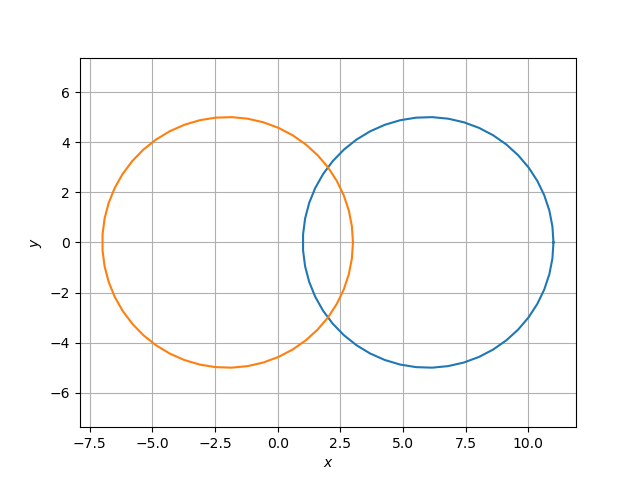
\includegraphics[scale=0.5]{conic.png}
\caption{Parabola}
\label{fig:Parabola}
\end{figure}
\end{flushleft}
\end{flushleft}
\end{document}
\fi
